We start by showing the result of the computation using the full matrices in order to see the image processing result.
We limit ourselves to grayscale images for the beginning.
As stated before, computing the entire matrices can only be done on small images.
The image below contains 135 000 pixels, so each matrix needs around 145 GB.

\begin{figure}[H]
 \centering
 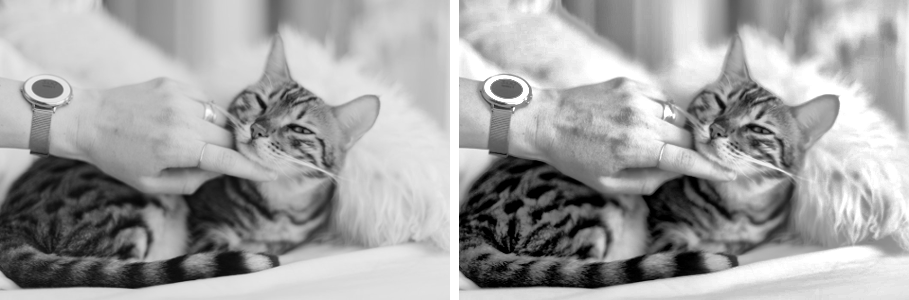
\includegraphics[width=0.95\textwidth]{img/cat.png}
 \caption{Left: input image. Right: sharpened image.}
 \label{fig:entire_result}
\end{figure}

As figure \ref{fig:entire_result} shows, the cat's fur on the left-hand side, the person's hand and the cushion on the right-hand side appear to be more detailed.
We observe that the already sharp part of the image, such as the cat's head, stays nice and is not over-sharpened.
We obtained this filter by defining \(f(\Lapl) = -3\Lapl\) in the output image \(z = (I - f(\Lapl))y\).

This corresponds to the adaptive sharpening operator defined in \cite{siam_slides_2016} as \((I + \beta \Lapl)\) with \(\beta > 0\).
This approach remains a simple application of a scalar and doesn't require any eigenvalue computation.
\ifthesis
 A more complete approach is called multiscale decomposition \cite{talebi_nonlocal_2014} and consists of applying a polynomial function to the Laplacian \(\Lapl\).
 It applies various coefficients to different eigenvalues of \(\Lapl\) because each eigenpair captures particular features of the image.
\fi
